% You should title the file with a .tex extension (hw1.tex, for example)
\documentclass[a4paper, 12pt]{report}

\usepackage{amsmath}
\usepackage{amssymb}
\usepackage{tabularx}
\usepackage{fancyhdr}
\usepackage{minted}
\usepackage{amsthm}        
\usepackage{graphicx}
\usepackage{hyperref}
\hypersetup{
    colorlinks=true,
    linkcolor=black,
    filecolor=magenta,      
    urlcolor=cyan,
    pdfpagemode=FullScreen,
}

\renewcommand\qedsymbol{$\blacksquare$}


\graphicspath{ {./pictures} }

\usepackage[margin=1in]{geometry}

\newcommand{\question}[2] {\vspace{.25in} \hrule\vspace{0.5em}
\noindent{\bf #1: #2} \vspace{0.5em}
\hrule \vspace{.10in}}
\renewcommand{\part}[1] {\vspace{.10in} {\bf (#1)}}

\newcommand{\myname}{Krittin Nisunarat}
\newcommand{\myhwnum}{1}
\newcommand{\mySubject}{ICCS315 Applied Algorithms}

\setlength{\parindent}{20pt}
\setlength{\parskip}{5pt plus 1pt}
 
\pagestyle{fancyplain}
\lhead{\fancyplain{}{\textbf{HW} \myhwnum}}      % Note the different brackets!
\rhead{\fancyplain{}{\myname}}
\chead{\fancyplain{}{\mySubject}}

\title{
	{
\includegraphics[width=80mm,scale=0.5]{MUIC_Logo_Eng_Center.png}} \\
	{\textbf{\mySubject}}\\
	{\large Assignment \myhwnum \ Report}\\
}
\author{
	{\textbf{Written by}} \\ 
	{Krittin Nisunarat 6280782}
}
\date{30 Jan 2022}
\thispagestyle{plain}


\begin{document}
\maketitle
\tableofcontents

\chapter{Resizeable Arrays}

Traditionally, resizable array has a high amortized cost depending on $\alpha$ for expansion and shrinking. HAT array theoretically fares
with a constant amortized cost on expansion and shrinking. Our goal is to perform teh benchmarking of the actual implementation of 
traditionaly resizable array and Sitarski's HAT array.

\section{Set up}

Both of data structure implementations are written in C++ which runs on ubuntu server. 
The actual implement is in \href{https://github.com/sudo-lucifer/applied-algo-hw1/tree/main/hat_array}{Github}.

\section{Append latency}

In this section, the cost of appending one key to the array mainly comes from reading memory. 
On tradditional resizable array, pushing new key to the back costs approximatetly 47 cycles
from reading memory pointer which needs to be conducted at most the entire array. On the other hand,
Sitarski's HAT array takes less cycle per apeend operation which is 26 cycles since the entire array is separated 
into $b$ size where $b$ where $b = 2^k$.

\begin{figure}[h]
        \centering
        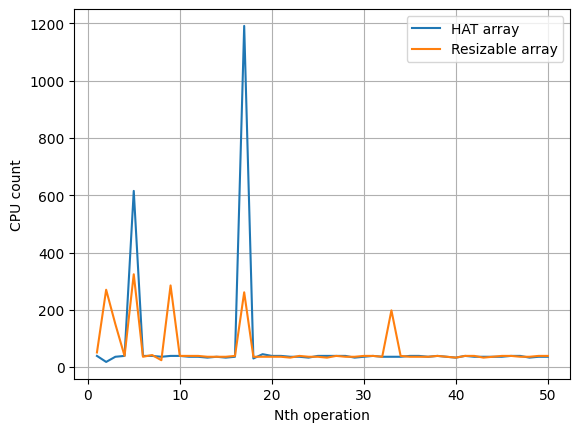
\includegraphics[width=0.4\textwidth,scale=0.2]{append_latency_output.png}
        \caption{\label{fig:append-latency} Benchmark of each append costs}
\end{figure}

Figure \ref{fig:append-latency} shows the cost of each append out of 50 append operations.
Tradditional resizable array shows up to stike CPU cycle more on each operation since the expansion
happens more often than HAT array. However, HAT array costs significantly higher cycle because the 
resizing needs to be done in both levels combine with copying data over.

In conclusion, traditional resizable array takes more cycle to access memory and append new day than
HAT array. On the expansion, tradditional resizable array is better than HAT array.

\section{Access latency}

Getting element by index in HAT array is tricky in the way that we need to calculate the block index and 
the index of element in particular block. This seems to take more cycle than traditional resizable array. 
Surprisingly, HAT array uses slightly less cycle then resizable array.
Benchmark is finding the average (out of 100,000 times) CPU count on each data structure element access. The result
is that HAT array takes 33 cycles on average while traditional resizable array takes 38 cycles. Therefore,
HAT array access element faster by 8 percents approximately.

\section{Scan throughput}

Continue from section 1.2, this section will illustrate the total latency of accesing/reading all elements
in array. Let's start with both arrays have 500 elements. HAT array costs 16800 cycles in total while 
traditional resizable array costs 18918 cycles on reading.

\begin{figure}[h]
        \centering
        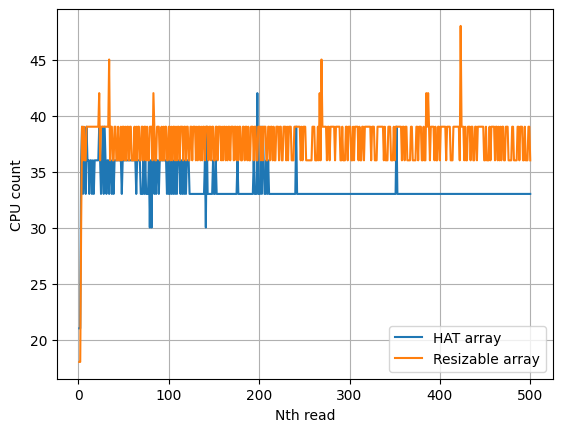
\includegraphics[width=0.4\textwidth,scale=0.2]{scan_output.png}
        \caption{\label{fig:scan-latency} Benchmark of scanning through array}
\end{figure}

As we can see in figure \ref{fig:scan-latency}, HAT array is nearly stable on reading after 300 elements.
Resizeable array, on the other side, have a few operation that strike CPU cycle which reaches over 45 cycles.
In conclusion, HAT array still wins in this competition that it scans faster by 13 percents.

\section{Overall throughput}

In section 1.1, I have shown append latency which conclude to have different benefits.
For this benchmark, I will test inserting 50 elements to both tradditional resizable array and
HAT array. As a consequence, resizable array takes 1153 cycles on average while HAT array takes
1114 cycles on average. Even though the expansion is costly in HAT array, overall throughput
of it is around 5 percents faster than resizable array.


\chapter{Skip lists}

\chapter{(a,b) tree}

\section{Multiple keys insertion.}

Starting with an empty tree, we want to insert the following keys:
\begin{center}
        733, 703, 608, 846, 309, 269, 55, 745, 548, 449, 513, 210, 795, 656, 262
\end{center}

The result of \emph{(2,3) tree} is

\begin{figure}[h]
        \centering
        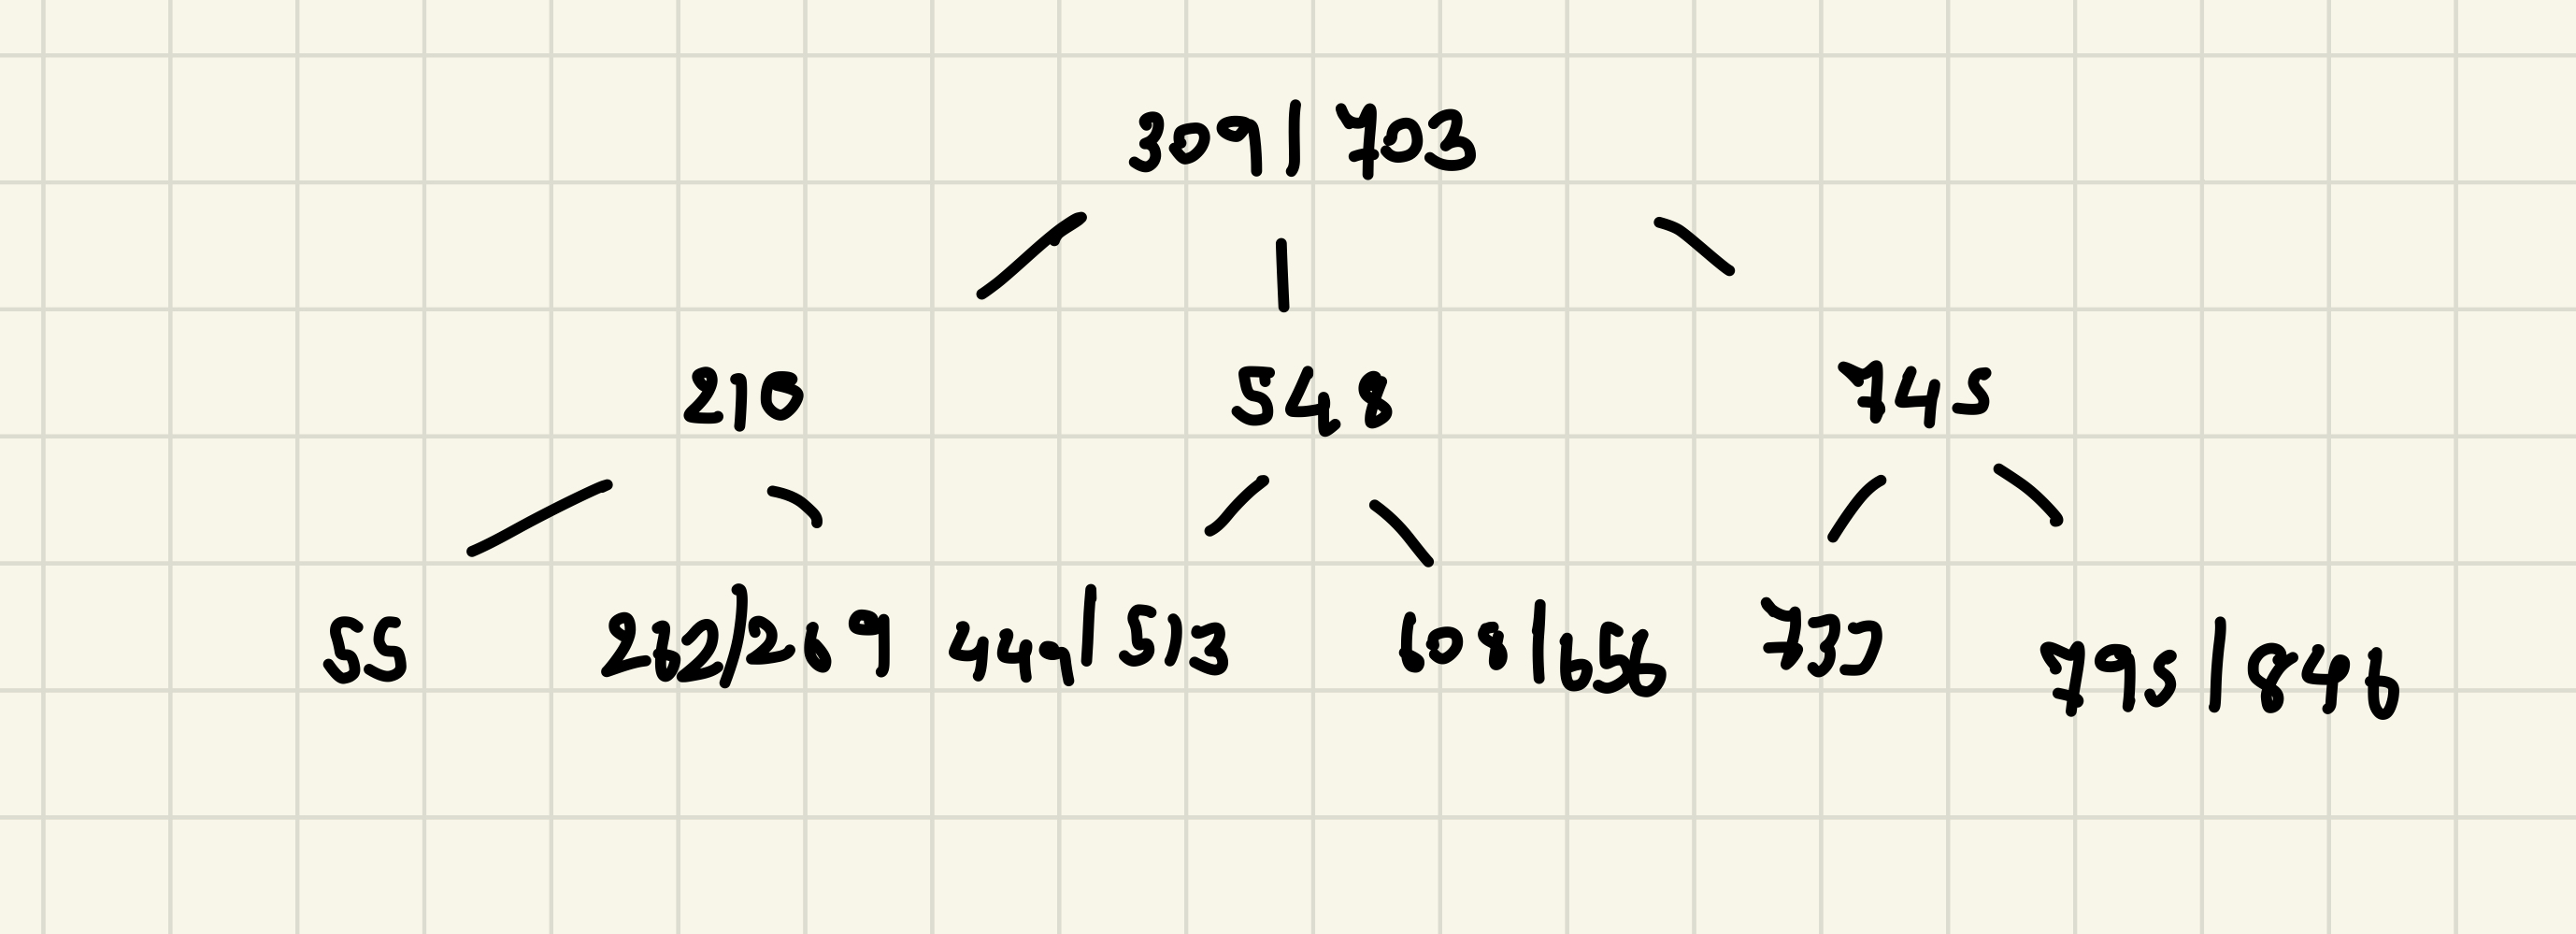
\includegraphics[width=0.8\textwidth,scale=0.5]{tree_insertion.jpeg}
\end{figure}

\section{Key deletion}

\noindent Suppose that we want to delete 309 in \emph{(2,3) tree} (Firgure \ref{fig:tree-deletion-1}), it falls into case 2 which 
we need to merge from sibling (Figure \ref{fig:tree-deletion-2}).

\begin{figure}[h]
        \centering
        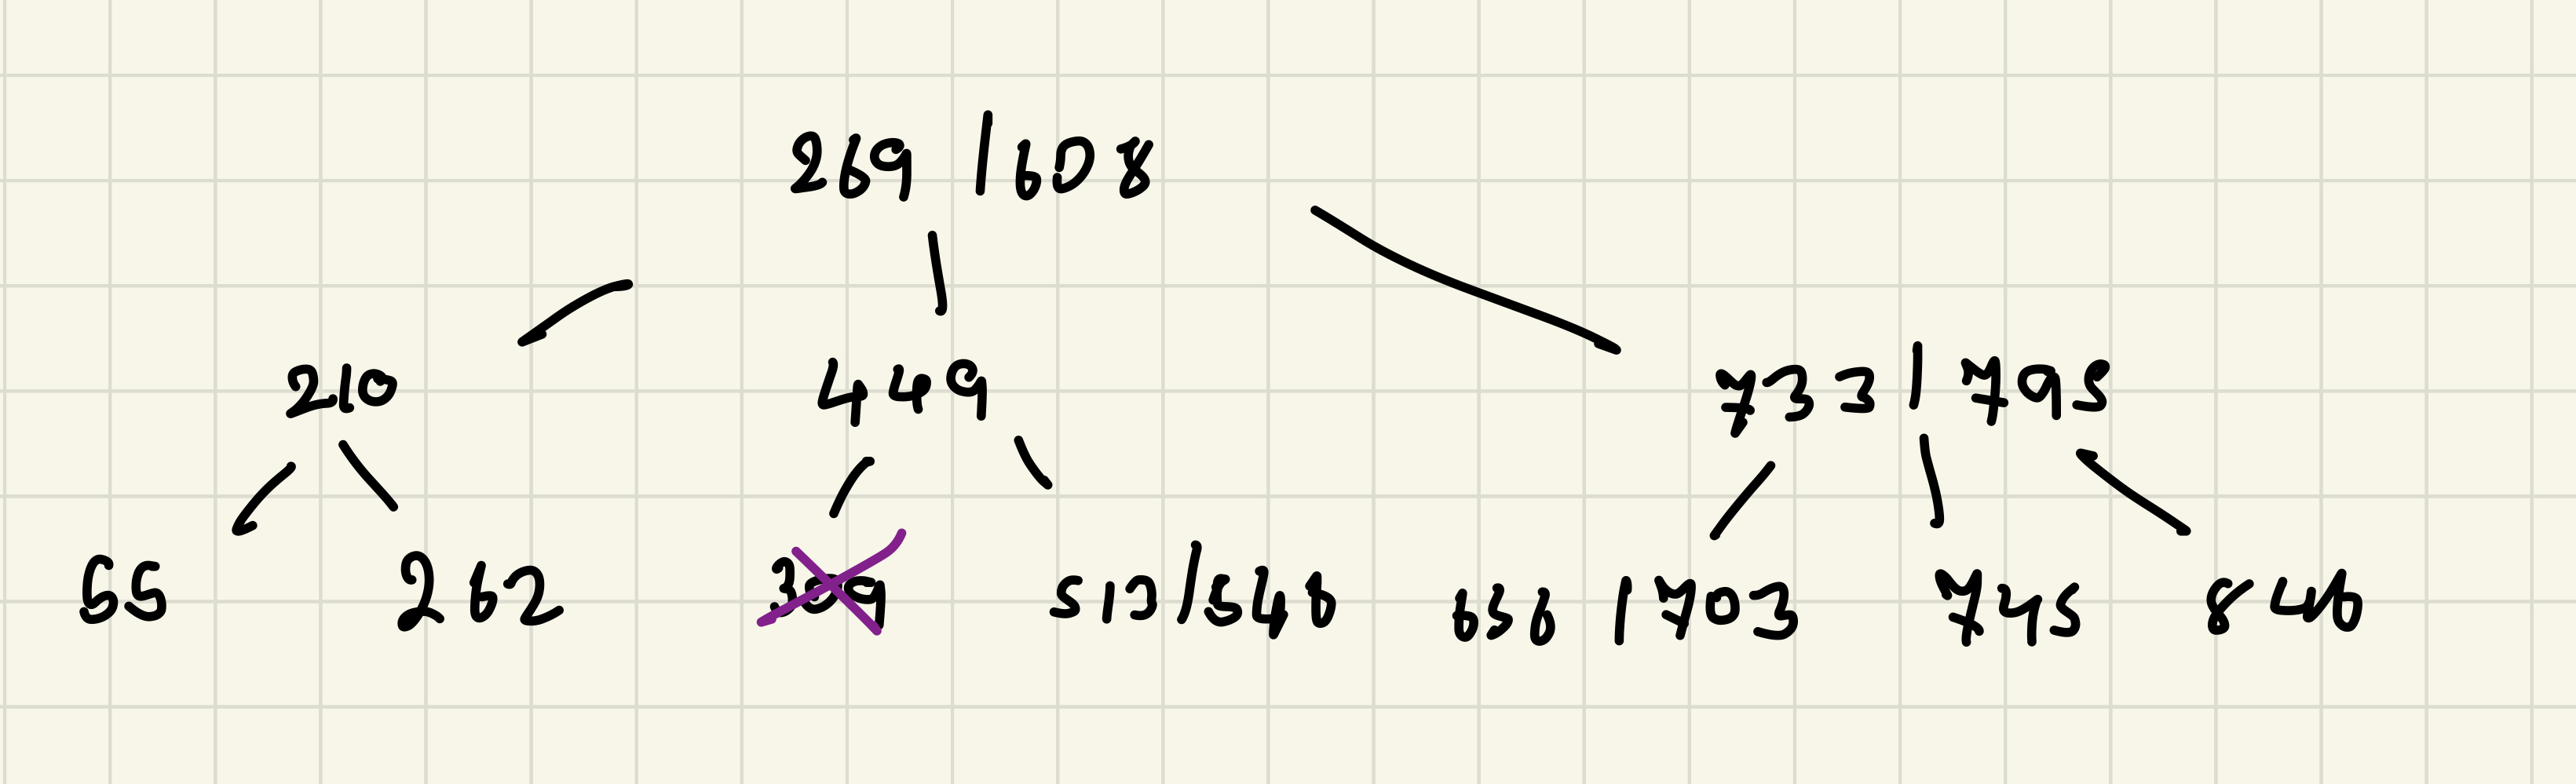
\includegraphics[width=0.7\textwidth,scale=0.5]{tree_deletion_1.jpeg}
        \caption{\label{fig:tree-deletion-1} Unbalanced tree without key 309}
\end{figure}

\begin{figure}[h]
        \centering
        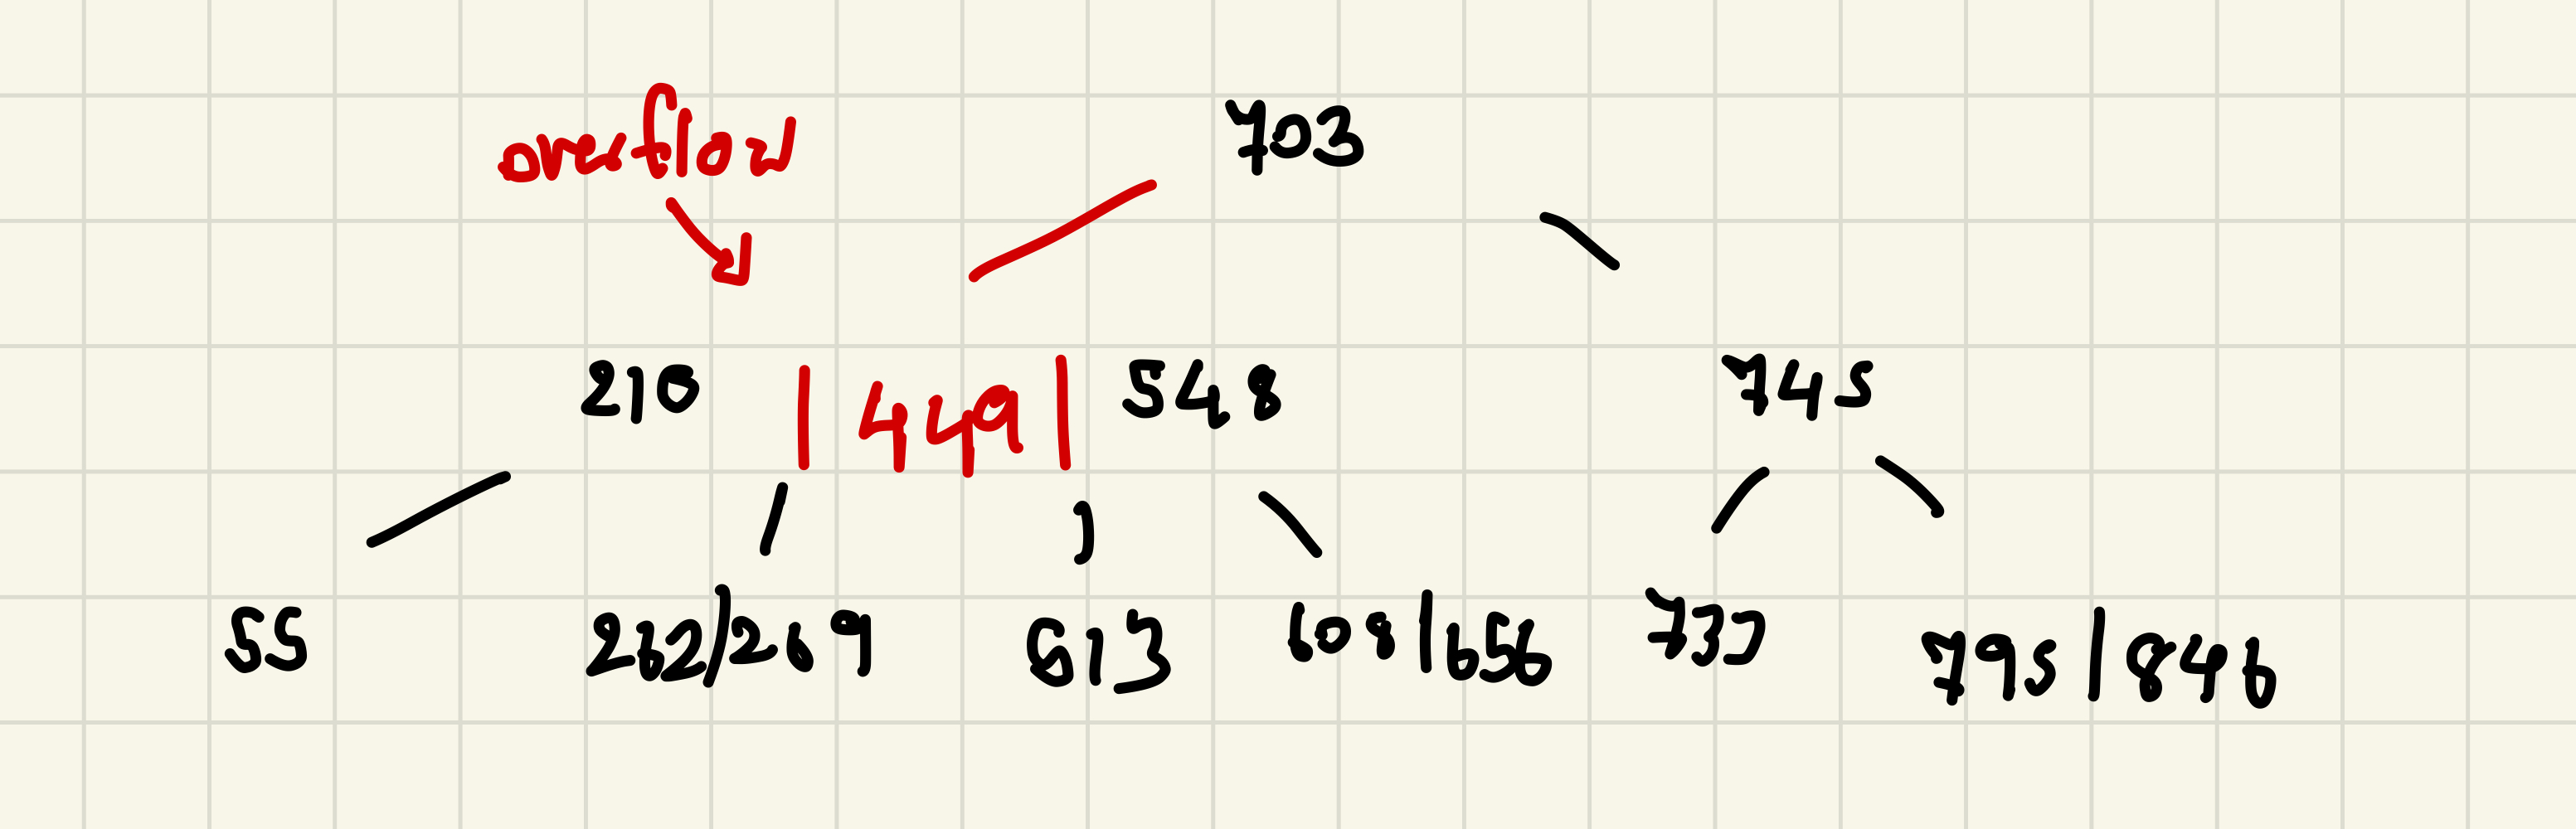
\includegraphics[width=0.8\textwidth,scale=0.5]{tree_deletion_2.jpeg}
        \caption{\label{fig:tree-deletion-2} Tree after merging}
\end{figure}

However, the merged tree in figure \ref{fig:tree-deletion-2} is not balance as the second layer node has 3 keys. So, we need to project 449 up to root.

\begin{figure}[h]
        \centering
        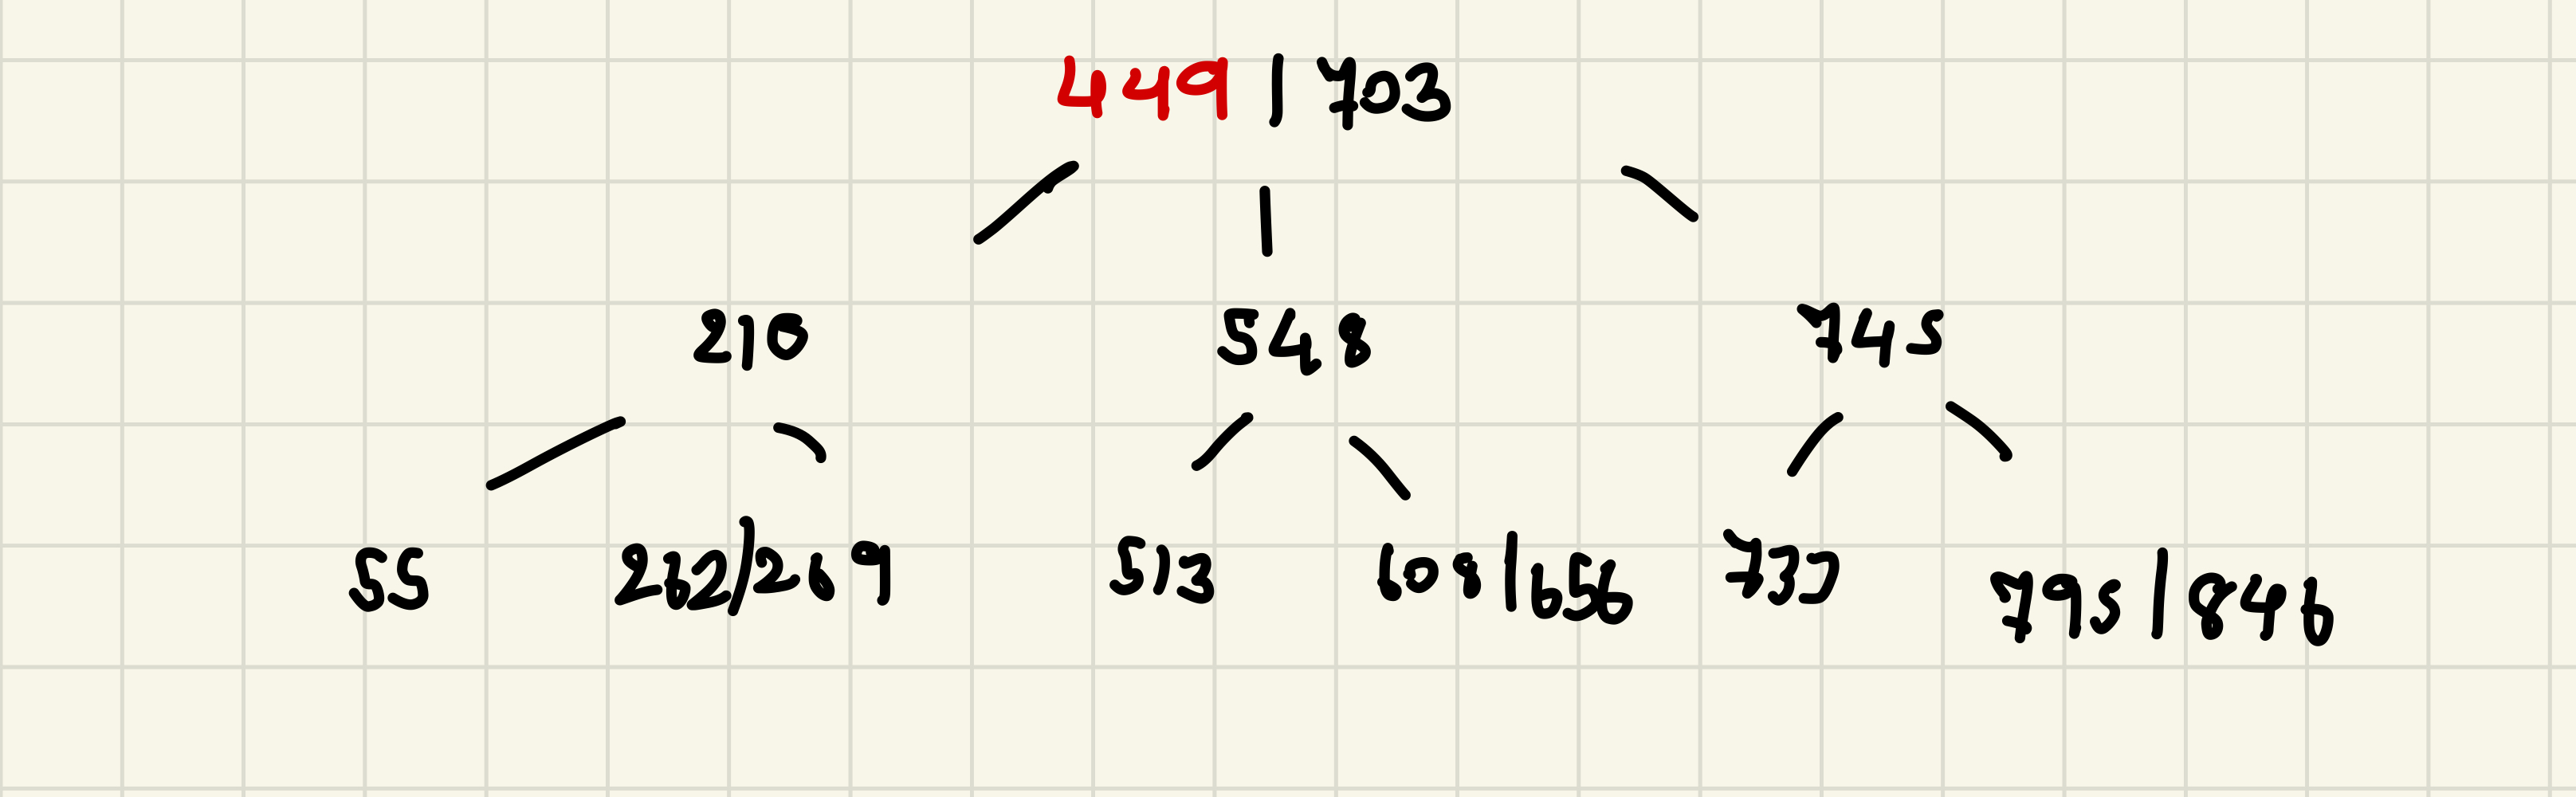
\includegraphics[width=0.8\textwidth,scale=0.5]{tree_deletion_3.jpeg}
        \caption{\label{fig:tree-deletion-3} Final tree}
\end{figure}


As you can see in Figure \ref{fig:tree-deletion-3}, the replacements are 449 which is the result from merging 
non-root tree in figure \ref{fig:tree-deletion-2}.
\begin{align*}
        \alpha_{\text{me}} &= a - 1 \\
        \alpha_{\text{sib}} &= a \\
        \alpha_{\text{sib}} + \alpha_{\text{me}} &= 2a - 1 \leq b
\end{align*} 


\chapter{B-tree speed}
\end{document}
